\documentclass{beamer}

% Draft (faster compilation, no images)
%\documentclass[draft]{beamer}

% Notes on the right
%\usepackage{pgfpages}
%\setbeameroption{show notes on second screen=right}

% Handout, no overlays
%\documentclass[handout]{beamer}

%\usepackage[utf8]{inputenc}
\usepackage[english]{babel}

\usetheme[
%  sectionpage=none,
  subsectionpage=none,
  numbering=none,
  progressbar=foot
]{metropolis}
\usecolortheme{owl} % Dark theme
\setmonofont{Inconsolata}
\definecolor{PowerDNSOrange}{RGB}{233,102,25}

% Some Open-Xchange colors
\definecolor{OXOrange}{RGB}{230,110,0}
\definecolor{OXGraphiteBlack}{RGB}{45,45,45}
\definecolor{OXSilverGrey}{RGB}{220,220,220}
\definecolor{OXGrey}{RGB}{135,135,135}

\definecolor{ProgressBarBG}{RGB}{238,238,236}
\setbeamercolor{progress bar}{fg=PowerDNSOrange, bg=OXGrey}

% Webicons
\usepackage{fontawesome}

\usepackage{shellesc}
\usepackage{minted}
\usemintedstyle{native}
\setminted[lua]{
  linenos=true,
  breaklines=true,
  frame=lines,
  fontsize=\footnotesize
}
\setminted[shell]{ % used for output
  style=bw,
  fontsize=\tiny
}
\renewcommand{\theFancyVerbLine}{\ttfamily
  \textcolor[rgb]{0.5,0.5,1.0}{\scriptsize
  \arabic{FancyVerbLine}}}

% Non-retarded image import
\usepackage{graphicx}

% PDF niceness
\usepackage{hyperref}

% No nav symbols on the PDF
\beamertemplatenavigationsymbolsempty

\title[aname]{ANAME: Address-specific DNS Name Redirection (draft-hunt-dnsop-aname)}
\author{\textbf{Peter van Dijk}\\PowerDNS Engineer\\with Evan Hunt and Anthony Eden}
\date{}
\titlegraphic{
  \vfill\large{\faicon{twitter-square}~Habbie\hfill Habbie~\faicon{github-square}}\\
              \small{\faicon{twitter-square}~PowerDNS\hfill PowerDNS~\faicon{github-square}}\\
              \vspace{150px}
              \center{
\includegraphics[width=.4\textwidth]{img/powerdns-logo.eps}}
}

\hypersetup{
  pdfauthor={Peter van Dijk},
  pdfsubject={},
  pdftitle={ANAME: Address-specific DNS Name Redirection},
  pdfkeywords={ANAME dns dnsop}
}

\begin{document}

\begin{frame}
  \titlepage
\end{frame}

\begin{frame}[fragile]{Why ANAME?}
  \begin{minted}[fontsize=\large]{shell}
$ORIGIN example.com.
@   IN SOA   ...
@   IN NS    ns1
@   IN A     192.0.2.1
www IN CNAME example.com.my-cdn.example.net.
  \end{minted}
\end{frame}

\begin{frame}{Current solutions}
  \begin{enumerate}
    \item CNAME at apex
    \item CNAME flattening
    \item cron updates
    \item ALIAS or ANAME from various commercial operators
    \item ALIAS in open source PowerDNS auth
  \end{enumerate}
\end{frame}

\begin{frame}{Creating a single standard}
  \center{
    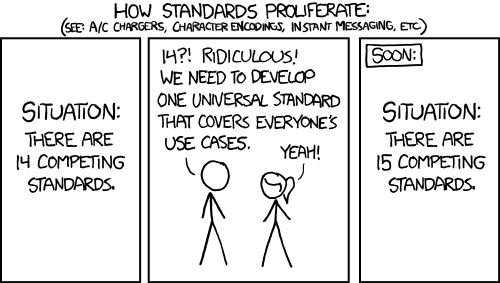
\includegraphics[width=.95\textwidth]{img/xkcd-standards.png}
  }
\end{frame}

\begin{frame}[fragile]{Usage}
  \begin{minted}[fontsize=\large]{shell}
$ORIGIN example.com.
@   IN SOA   ...
@   IN NS    ns1
@   IN ANAME example.com.my-cdn.example.net.
www IN CNAME example.com.my-cdn.example.net.
  \end{minted}
\end{frame}

\begin{frame}[fragile]{Remember CNAME?}
  \begin{minted}[fontsize=\normalsize]{shell}
;; QUESTION SECTION:
;www.example.com.   IN  A

;; ANSWER SECTION:
www.example.com. IN CNAME example.com.my-cdn.example.net.
example.com.my-cdn.example.net. IN A 198.51.100
  \end{minted}
\end{frame}

\begin{frame}[fragile]{Compare ANAME}
  \begin{minted}[fontsize=\normalsize]{shell}
;; QUESTION SECTION:
;example.com.   IN  A

;; ANSWER SECTION:
example.com.  86400 IN ANAME example.com.my-cdn.example.net.
example.com.  86400 IN A     198.51.100
  \end{minted}
\end{frame}

\begin{frame}{Concerns}
  \begin{itemize}
    \item DNSSEC
    \item loops
    \item GSLB
    \item TTL limiting/counting down
  \end{itemize}
\end{frame}

\begin{frame}{Questions?}
Questions? Comments?

(If you think this is a good idea, please let the IETF dnsop WG know, the call for adoption is open now!)
\end{frame}

\end{document}
